\documentclass[a4paper,10pt]{SMR}
\usepackage[utf8]{inputenc}
\usepackage{subcaption}
\usepackage{listings}
\usepackage{color}
\definecolor{codegreen}{rgb}{0,0.6,0}
\definecolor{codegray}{rgb}{0.5,0.5,0.5}
\definecolor{codepurple}{rgb}{0.58,0,0.82}
\definecolor{backcolour}{rgb}{0.95,0.95,0.92}
 
\definecolor{lightgray}{rgb}{.9,.9,.9}
\definecolor{darkgray}{rgb}{.4,.4,.4}
\definecolor{purple}{rgb}{0.65, 0.12, 0.82}

\lstdefinelanguage{JavaScript}{
  keywords={typeof, new, true, false, catch, function, return, null, catch, switch, var, if, in, while, do, else, case, break},
  keywordstyle=\color{blue}\bfseries,
  ndkeywords={class, export, boolean, throw, implements, import, this},
  ndkeywordstyle=\color{darkgray}\bfseries,
  identifierstyle=\color{black},
  sensitive=false,
  comment=[l]{//},
  morecomment=[s]{/*}{*/},
  commentstyle=\color{purple}\ttfamily,
  stringstyle=\color{red}\ttfamily,
  morestring=[b]',
  morestring=[b]"
}

\lstset{
   language=JavaScript,
   backgroundcolor=\color{lightgray},
   extendedchars=true,
   basicstyle=\footnotesize\ttfamily,
   showstringspaces=false,
   showspaces=false,
   numbers=left,
   numberstyle=\footnotesize,
   numbersep=9pt,
   tabsize=2,
   breaklines=true,
   showtabs=false,
   captionpos=b
}

\lstdefinestyle{mystyle}{
    backgroundcolor=\color{backcolour},   
    commentstyle=\color{codegreen},
    keywordstyle=\color{magenta},
    numberstyle=\tiny\color{codegray},
    stringstyle=\color{codepurple},
    basicstyle=\footnotesize,
    breakatwhitespace=false,         
    breaklines=true,                 
    captionpos=b,                    
    keepspaces=true,                 
    numbers=left,                    
    numbersep=5pt,                  
    showspaces=false,                
    showstringspaces=false,
    showtabs=false,                  
    tabsize=2
}
 
\lstset{style=mystyle}

\def\BibTeX{{\rm B\kern-.05em{\sc i\kern-.025em b}\kern-.08em
    T\kern-.1667em\lower.7ex\hbox{E}\kern-.125emX}}
    
%opening
\title{The SMR Website\\A client-searchable web index for SMR Articles}
\author{Nicholas J Bailey}
\smrtitle{The SMR Website}
\smrauthor{Nick Bailey}
\smraffiliation{SMRG Glasgow}
\begin{document}

\maketitle

% \begin{abstract}
% 
% \end{abstract}

\section{Setting Up}
\lstset{caption={Javascript from \texttt{index.html} with configuration options},label=l:configopts}
\begin{lstlisting}
<script>
// The title of the SMR as it appears in bibtex citations
var journalTitle = 'Scottish Music Review';

// Place where PDFs get stored
var docBase = 'http://place.where.pdfs.are';

// Edit the numbers and titles of all the volumes offered in the search dialogue.
//
// The first entry will always be interpreted as "All".
// The volumes will be presented in the order they appear in the list.
// For each volume:
//		The first item is the appearance in the pull-down menu;
//    The second item is the year of publication used for the bibtex citation;
//    The third item is the volume as stored in the bibtex citation;
//		The fourth item is the number as stored in the bibtex citation (may be null).
var volumes = [
	['4(2): Composition in the Post-Truth Age', '2019', '4', '2'],
	['4(1): Interdisciplinarity', '2014', '4', '1'],
	['3: Cultural Politics, inter alia', '2013', '3', null],
	['2(1): Popular and Reigious Music, et al', '2011', '2', '1'],
	['1(1): From the Scottish Universities', '2007', '1', '1']
]; 

\end{lstlisting}

\subsection{Initial Setup}
\label{s:setup}

Listing~\ref{l:configopts} shows the part of the file \texttt{index.html}
in the server's htdocs directory which must be configured to allow the web
site to work properly. Along with the \texttt{bibliography.bib} file, it
permits the generation of searchable indices of SMR volumes which are
processed in the web client, so that results are displayed without further
interaction with the SMR web server.

\begin{description}
 \item[journalTitle:] The full title of the journal which is used in the
 generation of copyable \BibTeX{} citations.
 \item[docBase:] The fully-qualified path to the root of the document archives.
 This is used to generate the download URLs, which are also presented as part
 of the copyable \BibTeX{} citations. The URL used to serve the documents
 MAY be different from that used to serve the web pages.
 \item[volumes:] Each volume published by the SMR has an entry in this array.
 The entries are used to sort by volume and to produce citations.
 The preceeding comment shows what each sub-entry indicates.
 
 Note that in the event there is no \texttt{number}, the 4th field MUST
 nonetheless be present and contain the special value \texttt{null}
 (\emph{not} \texttt{'null'}).
 
 Order is important; it is the order presented on the web page in the
 pull-down volume selection box. The default is to display only the top
 entry. This should therefore be the most recent published volume.
 The user may, however, elect to extend a search across all volumes.
\end{description}

Remember that elements of an array are \emph{separated} by a comma,
not terminated by one. Hence there is no comma before the bracket.

\subsection{Additional title-page content}

Place-holder HTML \texttt{$<$div$>$}s are provided for a navigation menu,
journal header and journal footer. These SHOULD be filled in with
appropriate content. The styles used to render the content MUST
be added to \texttt{css/smr.css} or to another file in that directory
which will have to be created and linked.

\subsection{The Bibliography}

\lstset{caption={A Sample Bibliography Entry},label=l:bibentry}
\begin{lstlisting}
@article{smr4bailey.south.evens.hair,
author={Bailey, Nicholas J and South, Alex and Evans, William and Hair, Graham},
title={A Microtonal Wind Controller},
volume={4},
number={1}
}
\end{lstlisting}
All of the SMR articles are maintained in a single \BibTeX{}
file called \texttt{bibliography.bib} which MUST be located in
the same folder as \texttt{index.html}. An example bibliography
entry is shown in Listing~\ref{l:bibentry}. Each of the \BibTeX{}
fields is complete and uses standard syntax. The \texttt{number}
entry MAY be omitted. The \texttt{journal}, \texttt{year} and \texttt{url}
entry MAY and should be omitted as they will in any case be ignored:
the journal title specified in the \texttt{index.html} file
will be used regardless; the year will be deduced from the
\texttt{volumes} array; the \texttt{url} will be set to reflect
the targeted file to be obtained when the title is clicked. 

Order of the entries in the bibliography file is preserved when
links to documents are generated and presented to the user.
The most recently published entries SHOULD therefore be placed
at the top of the bibliography file. Ordering of the entries
within the same volume MAY be arbitrary, or MAY at the editors'
discretion determine the ordering of titles within an on-line
volume.

\section{Presentation}

\begin{figure}
 \begin{subfigure}[t]{0.6\textwidth}
  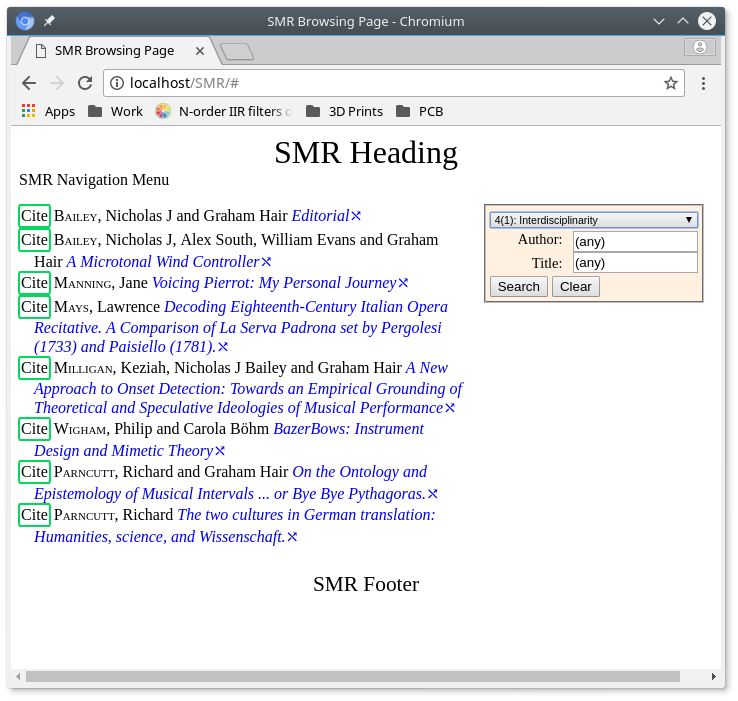
\includegraphics[width=\textwidth]{SMR_page-wide.png}
  \subcaption{Wider screens}
  \label{sf:wider}
 \end{subfigure}
 \begin{subfigure}[t]{0.3\textwidth}
  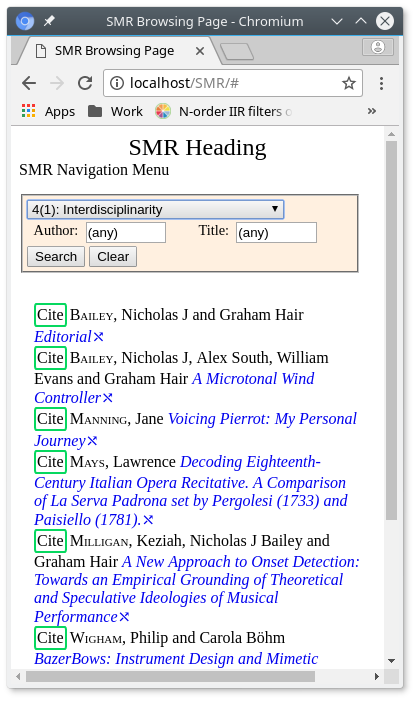
\includegraphics[width=\textwidth]{SMR_page-narrow.png}
  \subcaption{Narrower screens}
  \label{sf:narrower}
 \end{subfigure}
 \caption{Layout response on variation of screen width}
 \label{f:responsivelayout}
\end{figure}
The supplied style sheet takes advantage of \texttt{@media}
qualifies to determine the size of the display the user is reading.
Figure~\ref{f:responsivelayout} shows how the appearance of the site
changes as the geometry reduces.

Clicking the ``Cite'' button causes a generated bibliographic entry
to displayed which the user can copy and paste to their document
(Figure~\ref{f:cite}).
\begin{figure}
 \begin{center}
  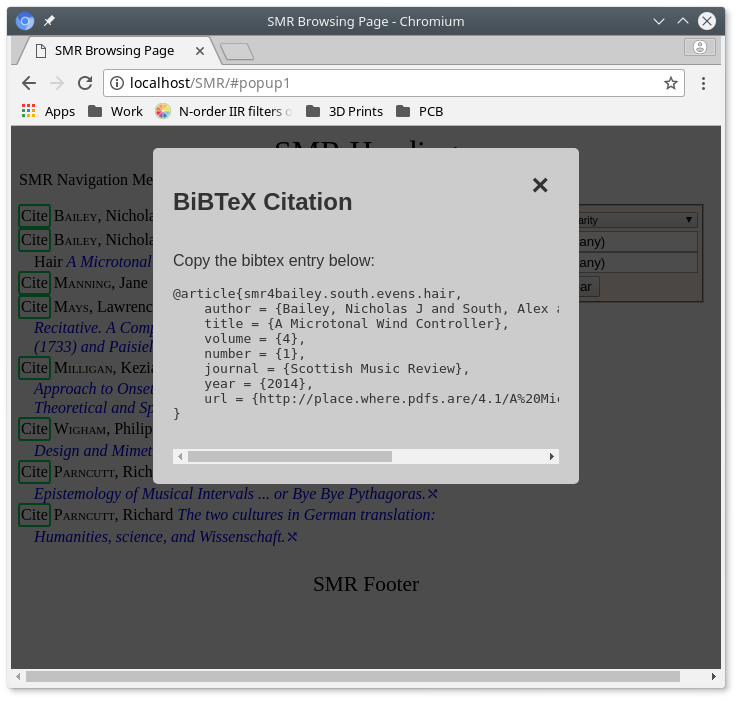
\includegraphics[width=0.6\textwidth]{SMR_page-citation.png}
 \end{center}
 \caption{\BibTeX{} citation produced on-demand}
 \label{f:cite}
\end{figure}

\begin{figure}
 \begin{subfigure}[t]{0.45\textwidth}
  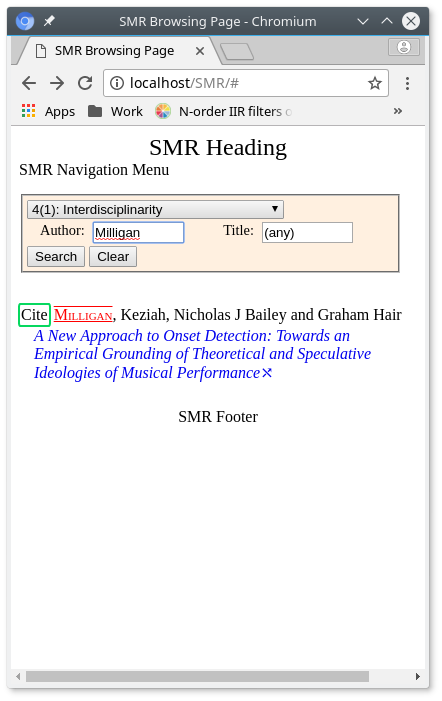
\includegraphics[width=\textwidth]{SMR_page-search.png}
  \subcaption{Searching a specific volume}
  \label{sf:specificvol}
 \end{subfigure}
 \begin{subfigure}[t]{0.45\textwidth}
  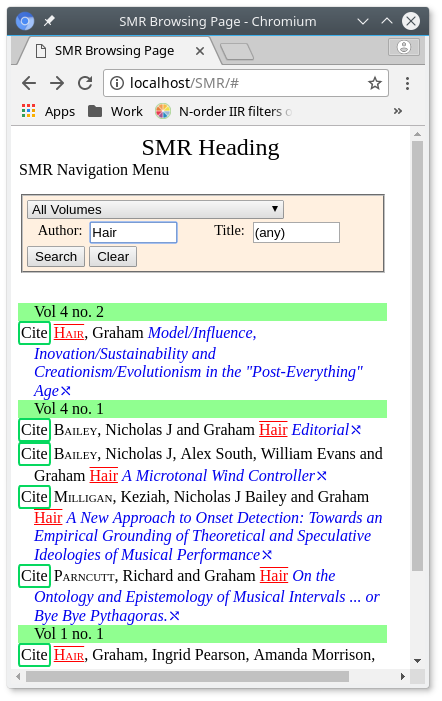
\includegraphics[width=\textwidth]{SMR_page-search-all.png}
  \subcaption{Searching all volumes}
  \label{sf:allvols}
 \end{subfigure}
 \caption{Result of searching for a particular author or title}
 \label{f:searchresult}
\end{figure}
When a search is performed, the matched terms are presented in highlight
as determined by the SMR style file. If the search is across all titles,
the volume and number of the matching title is displayed in a banner
across the result. See Figure~\ref{f:searchresult}.

\section{Storage of Files for Download}
Upon careful examination of the \BibTeX{} citation shown in
Figure~\ref{f:cite}, the form of the automatically generated
URL can be seen. It is constructed from the document root provided
in the \texttt{index.html} file (see Section~\ref{s:setup}),
the volume and number given in the bibliography file, and
a file name constructed from the document title.
The web administrator MUST ensure that the link thus
generated points to an accessible, well-formed document.

Since the solidus character (`/') is a directory separator,
it is replaced by a minus-sign when the document's title contains it.

\lstset{caption={Determination of linked URL from bibliographic data},label=l:bibToUrl}
\begin{lstlisting}
// Given the bibliographic data, generate the pdf document's escaped URI
function bibdataToURL(bibdata) {
	var url = docBase + '/' + bibdata.volume;
	if (typeof(bibdata.number) !== 'undefined')
		url += '.' + bibdata.number;
	var authors = bibdata['author'].split(' and ');
	var surnames = [];
	authors.forEach(function (author) {
		surnames.push(latexToUnicode(author.replace(/,.*/, '')))
	});
	url += '/' + 
		(surnames.join(', ') + ': ' + bibdata.title).replace(/\//g,'-') +
		'.pdf';
	return encodeURI(url);
}
\end{lstlisting}

The function responsible for calculating the URL from the bibliographic
details is as shown in Listing~\ref{l:bibToUrl}. As it stands, this produces
a URL containing the authors' surnames and title with spaces conserved.
This is considered reasonable, even though the file names produced can be
very long, because most clients select files using a pointing device
rather than having to type the complete filename. For example,

\begin{verbatim}
author = {Wigham, Philip and Carola B{\"o}hm},
title  = {BazerBows Instrument Design and Mimetic Theory},
volume = 4,
number = 1...
\end{verbatim}

produces the file path:

\noindent
\verb!4.1/Wigham, Böhm: BazerBows: Instrument Design and Mimetic Theory.pdf!

\section{Adding a New Page}

A file \verb!emptypage.html! is provided to ease the addition of new// Given the bibliographic data, generate the pdf document's escaped URI
function bibdataToURL(bibdata) {
	var url = docBase + '/' + bibdata.volume;
	if (typeof(bibdata.number) !== 'undefined')
		url += '.' + bibdata.number;
	var authors = bibdata['author'].split(' and ');
	var surnames = [];
	authors.forEach(function (author) {
		surnames.push(latexToUnicode(author.replace(/,.*/, '')))
	});
	url += '/' + 
		(surnames.join(', ') + ': ' + bibdata.title).replace(/\//g,'-') +
		'.pdf';
	return encodeURI(url);
}

pages to the site. To remove the dependency on the server to provide
particular language support, the supplied pages are simple copies of
the empty page with the necessary changes having been made.
The REQUIRED changes are:
\lstset{caption={Determination of linked URL from bibliographic data},label=l:navmenu}
\begin{lstlisting}
<div id="navMenu">
<!-- You have to add 'class="current"' to one navbutton's link -->
	<span class="navbutton"><a href="." />Home</a></span>
	<span class="navbutton"><a class="current" href="./about.html" />About</a></span>
	<span class="navbutton tooltip"><a href="./board.html" />
	  <span class="tooltiptext">Contact SMR Editorial Board</span>Board</a></span>
	<span class="navbutton tooltip">
		<span class="tooltiptext">Instructions for Authors</span>
		<a href="./submissions.html" />Submissions</a></span>
</div>
\end{lstlisting}
\begin{itemize}
 \item Add the page title to the HTML <title> element.
 \item Replace the main heading in the HTML <h1> element.
 \item Assert the current page in the navigation menu. Looking at Listing~\ref{l:navmenu},
 which shows the relevant part of the file \texttt{about.html}. The ``about'' button's
 link element. It has a class attribute declaring it to be of class ``current''
 whereas the others do not.
 \item Add the page content to the <div> element with the id attribute ``pageContent''.
 On the desktop, the page is divided into 12 columns. The width of a <div> can
 be specified as a multiple of these columns. When viewed on a small screen
 device, the <divs> will always appear vertically stacked.
 \item To change the web site copyright year, modify the \texttt{css/smr.css} file.
 The year copyright year will then appear modified on every page of the site.
\end{itemize}

\begin{figure}
 \begin{center}
  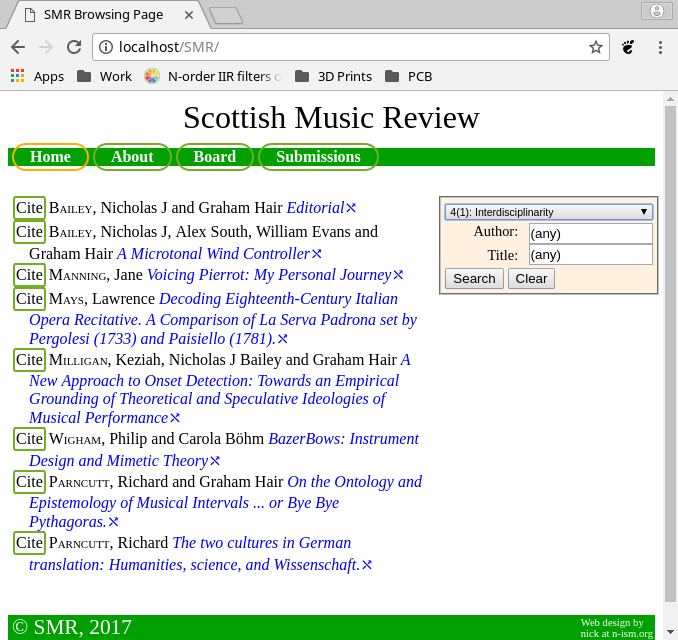
\includegraphics[width=0.8\textwidth]{navbar.png}
 \end{center}
 \caption{The main page integrated into the navigation menu}
 \label{f:navbar}
\end{figure}

This should result in a desktop screen with the appearance shown in
Figure~\ref{f:navbar}.
\end{document}
